% Source : http://tex.stackexchange.com/questions/18831/how-to-make-number-triangles

\documentclass{article}
	\usepackage{tikz}
	\usetikzlibrary{positioning,shadows,backgrounds}


\begin{document}

\centering

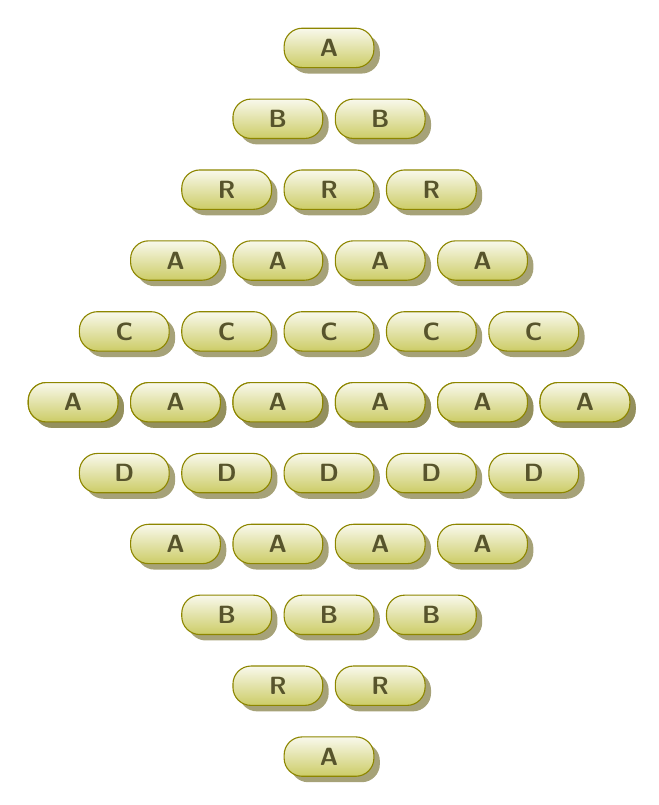
\begin{tikzpicture}[x=13mm,y=9mm]
	\tikzset{every node/.style={
		minimum height=5mm,
		inner sep=.7mm,
		text width=10mm,
		align=center,
		font=\small\bfseries\sffamily,
		text=olive!50!black,
		draw=olive,
		top color=olive!5,
		bottom color=olive!40,
		rounded corners=2.3mm,
		drop shadow={fill=olive!40!gray,fill opacity=.8}}
	}
	\foreach \row/\letterT/\letterB in {0/A/A,1/B/R,2/R/B,3/A/A,4/C/D,5/A} {
		\foreach \col in {0,...,\row}{
			\coordinate (pos) at (-\row/2+\col,-\row);
			\node at (pos) {\letterT};
			\coordinate (posB) at (-\row/2+\col,\row-10); % use: \row-2 times the max. value for \row
			\node at (posB) {\letterB};
		}
	}
\end{tikzpicture}

\end{document}
